Sabiendo como se expresó en la explicación cuál es el mejor y el peor caso, se construyeron archivos de prueba para los mismos. También hicimos uno con datos obtenidos de forma aleatoria. Luego obtuvimos los tiempos de ejecución y los graficamos en función de la entrada, como se puede ver a continuación:
\newline
Mejor caso:
\newline
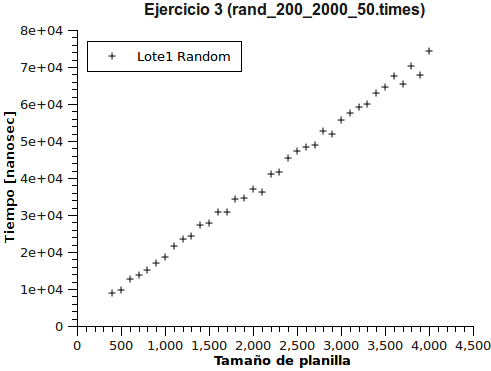
\includegraphics[scale=0.8]{img/ej1/Graph1.png}
\newline
Peor caso:
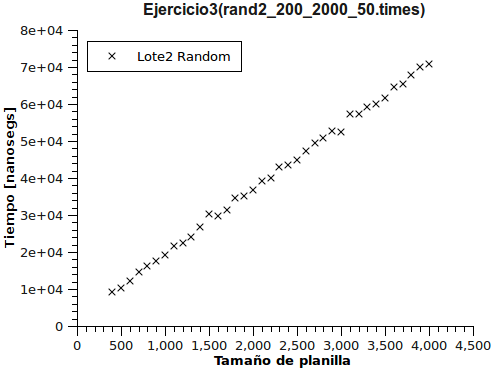
\includegraphics[scale=0.8]{img/ej1/Graph2.png}
\newline
Aleatorio:
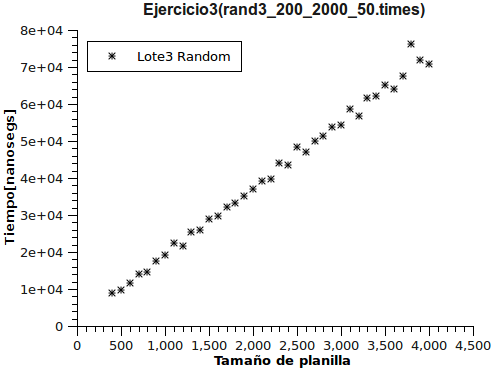
\includegraphics[scale=0.8]{img/ej1/Graph3.png}
\newline
